\section{Інфраструктура}

Для размяшчэння вэб-сайта электроннай бібліятэкі было вырашына выкарыстоўваць Amazon воблака, так як
яно прадастаўляе багатыя магчымасці для пабудовы інфраструктуры любога памеры і для любых мэт.

Amazon Web Services (AWS) --- гэта самая распаўсюджаная ў свеце воблачная платформа з найшырокімі магчымасцямі, якая прадстаўляе больш за 175 поўнафункцыянальных сeрвісаў для цэнтраў апрацоўкі даных па ўсёй планеце. Мільёны кліентаў (у тым ліку стартапы, якія сталі лідарамі па хуткасці росту, найбуйнейшыя карпарацыі і перадавыя ўрадавыя ўстановы) выкарыстоўваюць AWS для зніжэння выдаткаў, павышэння гнуткасці і паскоранага ўкаранення інавацый.

У AWS самая шырокая воблачная інфраструктура ў свеце. Ні адзін іншы правайдар воблачных сeрвісаў не ахоплівае столькі рэгіёнаў і зон даступнасці, злучаючы іх з нізкай затрымкай, высокай прапускной здольнасцю і надмернасцю рэсурсаў сеткі. AWS ўключае ў сябе 69 зон даступнасці, якія размешчаны ў 22 геаграфічных рэгіёнах па ўсім свеце. У найбліжэйшы час плануецца стварэнне яшчэ 13 зон даступнасці і чатырох рэгіёнаў AWS ў Інданэзіі, Італіі і Іспаніі. Мадэль рэгіёнаў і зон даступнасці AWS была рэкамендавана Gartner для запуску карпаратыўных праграм, якія патрабуюць высокай даступнасці.

На малюнку \ref{img: aws infra} прадстаўлена пабудаваная інфраструктура
для электроннай бібліятэкі ў Amazon воблаку.

\begin{figure}[h!]
    \centering
    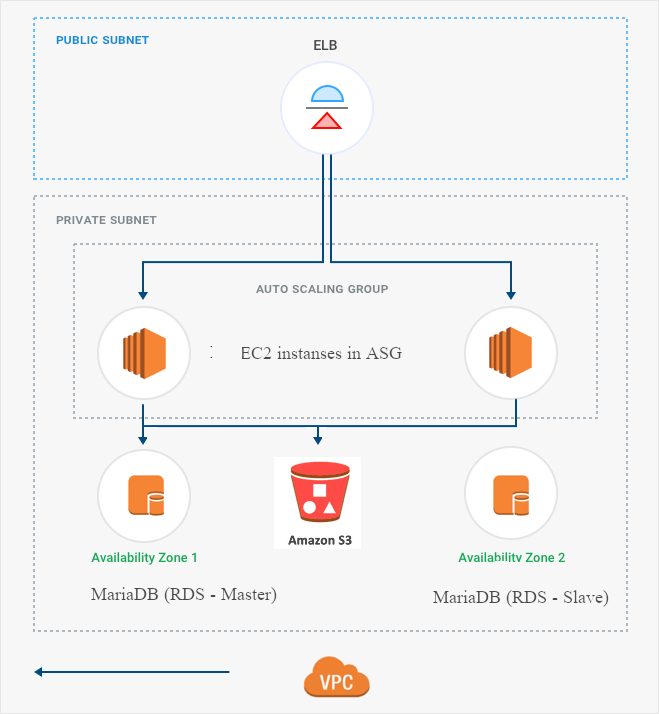
\includegraphics[width=0.6\textwidth]{aws}
    \caption{Інфраструктура электроннай бібліятэкі ў Amazon воблаку}
    \label{img: aws infra} 
\end{figure}

Для забеспячэння высокай даступнасці было вырашана выкарыстоўваць ASG (Auto Sca\-ling Group),
якія змяшчаюць EC2 (Elastic Compute Cloud) з устаноўленай праграмай, якая адказвае за логіку
сервіса электроннай бібліятэкі.

Так як у ASG можа быць разгорнута некалькі EC2 машын адначасова, неабходна забяспечыць адзіны
ўваход на сервіс. Для развязвання гэтай праблемы выкарыстоўваецца ELB (Elastic Load Balancer),
які дазваляе размяркоўваць трафік на любую колькасць машын у ASG.

Неабходна заўважыць, што для большай бяспекі EC2 машыны і RDS (Relational Database Service)
размяшчаюцца ў прыватнай сетцы, гэта значыць да іх немагчыма падключыцца з Інтэрнэта.
На ELB праслухоўваецца толькі адзін порт (80) па пратаколу HTTP, на якім працуе электронная бібліятэка.
Гэта дазваляе пазбегнуць несанкцыяванага падключэння да EC2 машын і знішэння сістэмы.
Да RDS сервіса мае магчымасць звяртацца з запытам толькі EC2 машыны, што забяспечвае высокі ўзровень
бяспекі ад незаконнага атрымання даных з базы даных.

Ніжэй будуць апісаны сервісы ELB, ASG, EC2, а сервісы S3 і RDS будуць апісаны ў раздзеле <<Сховішча даных>>.

\subsection{Elastic Load Balancer}

Elastic Load Balancing аўтаматычна размяркоўвае ўваходны трафік праграм па некалькіх мэтавых аб'ектах, такіх як Amazon EC2, кантэйнеры, IP-адрасы і Lambda функцыі. Ён можа размяркоўваць трафік праграмы ў адной зоне даступнасці або паміж некалькімі зонамі даступнасці. Elastic Load Balancing прапануе тры тыпы размеркавальнікаў нагрузкі, якія забяспечваюць высокую даступнасць, аўтаматычнае маштабаванне і надзейную абарону, неабходную для забеспячэння адмоваўстойлівасці праграм.

Так як электронная бібліятэка ўяўляе сабой вэб-сайт быў абраны тып Application Load Balancer.
Application Load Balancer лепш за ўсё падыходзіць для балансавання нагрузкі трафіку HTTP і HTTPS і забяспечвае пашыраную маршрутызацыю запытаў, арыентаваную на дастаўку праграм, якія пабудаваныя на базе сучасных архітэктур, уключаючы мікрасервісы і кантэйнеры. Працуючы на ўзроўні асобных запытаў (узровень 7), Application Load Balancer накіроўвае трафік на мэтавыя аб'екты ў Amazon Virtual Private Cloud (Amazon VPC), абапіраючыся на змест запыту.

\subsection{Auto Scaling Group}

AWS Auto Scaling Group выконвае маніторынг праграм і аўтаматычна настройвае рэсурсы для падтрымання стабільнай прагназуемай прадукцыйнасці пры мінімальна магчымых выдатках. AWS Auto Scaling Group дазваляе за лічаныя хвіліны проста наладзіць маштабаванне прыкладанняў для мноства рэсурсаў у розных сeрвісах. Сeрвіс валодае зручным і магутным карыстацкім інтэрфейсам, які дазваляе ствараць планы маштабавання для такіх рэсурсаў, як машыны і спотавыя групы Amazon EC2, задачы Amazon ECS, табліцы і індэксы Amazon DynamoDB, а таксама рэплікі Amazon Aurora. AWS Auto Scaling Group спрашчае маштабаванне за кошт рэкамендацый, якія дазваляюць аптымізаваць прадукцыйнасць, выдаткі або суадносіны паміж імі.

AWS Auto Scaling дазваляе падтрымліваць аптымальную прадукцыйнасць і даступнасць праграм, нават калі працоўныя нагрузкі з'яўляюцца перыядычнымі, непрадказальнымі або пастаянна змяняюцца. AWS Auto Scaling пастаянна выконвае маніторынг праграм, правяраючы іх узровень прадукцыйнасці на адпаведнасць устаноўленых значэнняў. Пры пікавай нагрузцы AWS Auto Scaling Group аўтаматычна павялічвае аб'ём рэсурсаў, тым самым падтрымліваючы высокую якасць сeрвісу.

AWS Auto Scaling Group здольны аптымізаваць выкарыстанне рэсурсаў і павысіць эканамічную эфектыўнасць прымянення сeрвісаў AWS, каб плаціць толькі за тыя рэсурсы, якія сапраўды патрабуюцца. Пры памяншэнні нагрузкі AWS Auto Scaling Group аўтаматычна вызваляе залішнія рэсурсы, каб пазбегнуць дадатковых выдаткаў. Сeрвіс AWS Auto Scaling Group прадастаўляецца бясплатна і дазваляе аптымізаваць выдаткі на AWS асяроддзе.

\subsection{Elastic Compute Cloud}

Amazon Elastic Compute Cloud (Amazon EC2) --- гэта вэб-сeрвіс, які прадастаўляе бяспечныя маштабуемыя вылічальныя рэсурсы ў воблаку. Ён дапамагае распрацоўнікам, спрашчаючы правядзенне вылічэнняў у воблаку ў маштабе ўсяго Інтэрнэту.

Amazon EC2 дазваляе павялічваць або памяншаць вылічальную магутнасць за некалькі хвілін, а не гадзін або дзён. Можна ўводзіць у эксплуатацыю адну серверную машыну, сотні ці нават тысячы серверных машын адначасова. Можна таксама выкарыстоўваць Amazon EC2 Auto Scaling, каб падтрымліваць даступнасць групы EC2 і аўтаматычна маштабаваць групу ў патрэбным кірунку ў залежнасці ад патрэбаў, каб падтрымліваць максімальную прадукцыйнасць і скарачаць выдаткі.

Сeрвіс дазваляе выбіраць розныя тыпы машын, аперацыйных сістэм і пакетаў ПЗ. У Amazon EC2 можна выбраць неабходны аб'ём памяці, колькасць працэсараў, аб'ём дыскавай падсістэмы, а таксама памер сістэмнай часткі, аптымальныя для аперацыйнай сістэмы і праграмы.
